\chapter{Lec 20 - Constraint Satisfaction Problems}
\section{Introduction}
When we talked about problem solving agents we explored the idea that problems can be solved by searching in a space of \textbf{states}. These states can be evaluated by domain-specific heuristics and tested to see whether they are goal states. From the point of view of the search algorithm, however, each state is
atomic, or indivisible, a black box with no internal structure.\\\\
This chapter describes a way to solve a wide variety of problems more efficiently. We use a \textbf{factored representation} for each state:  a set of variables, each of which has a value. A problem is solved when each variable has a value that satisfies all the constraints on the variable. A problem described this way is called a \textbf{constraint satisfaction problem}, or CSP.\\\\
CSP search algorithms take advantage of the structure of states and use general-purpose rather than problem-specific heuristics to enable the solution of complex problems. The main idea is to eliminate large portions of the search space all at once by identifying variable/value combinations that violate the constraints.

\section{Constraint satisfaction problems}
A constraint satisfaction problem consists of three components, $X$, $D$, and $C$:
\begin{itemize}
    \item $X$ is a set of variables, $\{X_1, ..., X_n\}$
    \item $D$ is a set of domains, $\{D_1, ..., D_n\}$, one for each variable.
    \item $C$ is a set of constraints that specify allowable combinations of values.
\end{itemize}
To solve a CSP, we need to define a state space and the notion of a solution. Each
state in a CSP is defined by an \textbf{assignment} of values to some or all of the variables. An assignment that does not violate any constraints is called a \textbf{consistent} or legal assignment. A \textbf{complete assignment} is one in which every variable is assigned, and a \textbf{solution} to a CSP is a consistent, complete assignment. A \textbf{partial assignment} is one that assigns values to only some of the variables.

\subsection{Example problem: Map coloring}
We are given the task of coloring each region of Australia  either red, green, or blue in such a way that no neighboring regions have the same color. To formulate this as a CSP, we define the variables to be the regions:
\[X = \{WA, NT, Q, NSW ,V, SA, T\}\]
The domain of each variable is the set $D_i = \{red, green, blue\}$. The constraints require neighboring regions to have distinct colors. Since there are nine places where regions border, there are nine constraints:
\[C = \{SA \neq WA, SA \neq NT, SA \neq Q, SA \neq NSW , SA \neq V,
WA \neq NT, NT \neq Q, Q \neq NSW , NSW \neq V \} .\]
There are many possible solutions to this problem, such as:
\[\{WA = red, NT = green, Q = red, NSW = green, V = red, SA = blue, T = green \}.\]
\begin{center}
    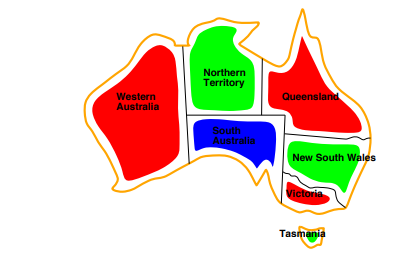
\includegraphics[]{images/CSP.png}
\end{center}
It can be helpful to visualize a CSP as a \textbf{constraint graph}, as shown in the figure below.
\begin{center}
    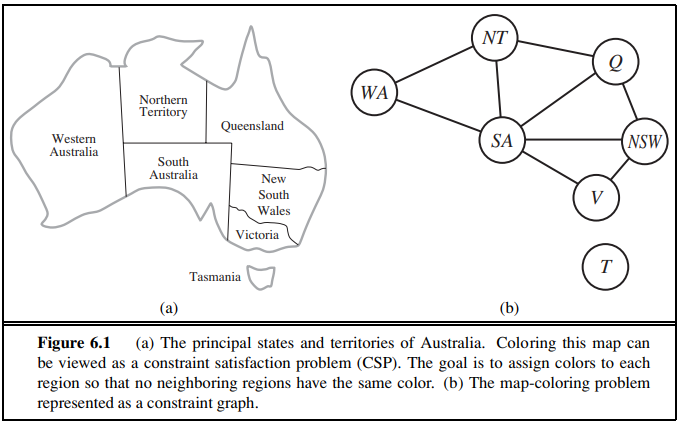
\includegraphics[scale=0.8]{images/CSP-constraint-graph.png}
\end{center}
The nodes of the graph correspond to variables of the problem, and a link connects any two variables that participate in a constraint. Note that this problem is a Binary CSP, that is, each constraint relates at most two variables.\\\\
CSP solvers can be faster than state-space searchers because the CSP solver can quickly eliminate large swatches of the search space. For example, once we have
chosen $\{SA = blue\}$ in the Australia problem, we can conclude that none of the five neighboring variables can take on the value blue. 

\section{Variations on the CSP formalism}
The simplest kind of CSP involves variables that have \textbf{discrete}, \textbf{finite domains}. 
\\\\
A discrete domain can be \textbf{infinite}, such as the set of integers or strings. With infinite domains, it is no longer possible to describe constraints by enumerating all allowed combinations of values. Instead, a \textbf{constraint language} must be used.
\\\\
Special solution algorithms (which we do not discuss here) exist for \textbf{linear constraints} on integer variables, that is, constraints in which each variable appears only in linear form. It can be shown that no algorithm exists for solving general \textbf{nonlinear constraints} on integer variables.  
\\\\
Constraint satisfaction problems with \textbf{continuous domains} are common in the real world and are widely studied in the field of operations research. The best-known category of continuous-domain CSPs is that of \textbf{linear programming} problems, where constraints must be linear equalities or inequalities. Linear programming problems can be solved in time polynomial in the number of variables.\\\\
In addition to examining the types of variables that can appear in CSPs, it is useful to look at the \textbf{types of constraints}:
\begin{itemize}
    \item The simplest type is the \textbf{unary constraint}, which restricts the value of a single variable. For example, in the map-coloring problem it could be $SA \neq green$.

    \item A \textbf{binary constraint} relates two variables. For example, $SA \neq NSW$ is a binary constraint.

    \item  We can also describe \textbf{higher-order constraints}, which involve 3 or more variables, such as asserting that the value of $Y$ is between $X$ and $Z$. An example of higher-order constraints problem is provided by \textbf{cryptarithmetic} puzzles.
    \begin{center}
        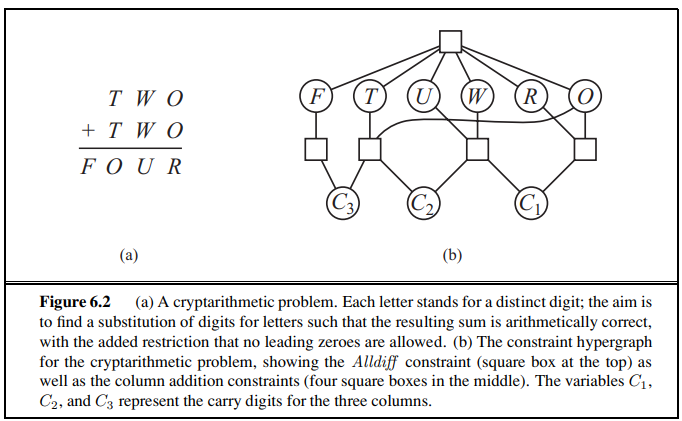
\includegraphics[scale=0.8]{images/CSP-ca.png}
    \end{center}

    \item  Many real-world CSPs include \textbf{preference constraints} indicating which solutions are preferred,  e.g., red is better than green, often representable by a cost for each variable assignment. With this formulation, CSPs with preferences can be solved with optimization search methods, either path-based or local. We call such a problem a \textbf{constraint optimization problem}, or COP. Linear programming problems do this kind of optimization.
\end{itemize}
Examples of Real-world CSPs:
\begin{itemize}
    \item Assignment problems e.g., who teaches what class
    \item Timetabling problems
    \item Hardware configuration
    \item Spreadsheets
    \item Transportation scheduling
    \item Factory scheduling
    \item Floorplanning
\end{itemize}
Notice that many real-world problems involve real-valued variables.

\section{Backtracking search}
In this section we look at \textbf{backtracking search} algorithms that work on partial assignments. Let’s start with the straightforward, dumb approach, then fix it. We could apply a standard depth-limited search. A state would be a partial assignment, and an action would be assign a value to an unassigned variable that does not conflict with current assignment. The goal test would be checking if the current assignment is complete. But for a CSP with $n$ variables of domain size $d$, we quickly notice something terrible:  the branching factor at the top level is $nd$ because any of $d$ values can be assigned to any of $n$ variables. At
the next level, the branching factor is $(n - 1)d$, and so on (branching factor at depth $l$ is $(n-l)d$). Therefore, we would generate a tree with $n! \cdot d^n$ leaves, even though there are only $d^n$ possible complete assignments!\\\\
Our naive formulation ignores crucial property common to all CSPs: \textbf{commutativity}.  CSPs are commutative because when assigning values to variables, we reach the same partial assignment regardless of order. Therefore, we
need only to consider assignments to a \textbf{single variable} at each node in the search tree. For example, at the root node of a search tree for coloring the map of Australia, we might make a choice between $SA = red, SA = green$, and $SA = blue$,  but we would never choose between $SA = red$ \textbf{and} $WA = blue$. With this restriction, the number of leaves is $d^n$, as we would hope. Depth-first search for CSPs with single-variable assignments is called \textbf{backtracking search}. Backtracking search is the basic uninformed algorithm for CSPs. It can solve n-queens for $n \approx 25$
\begin{center}
    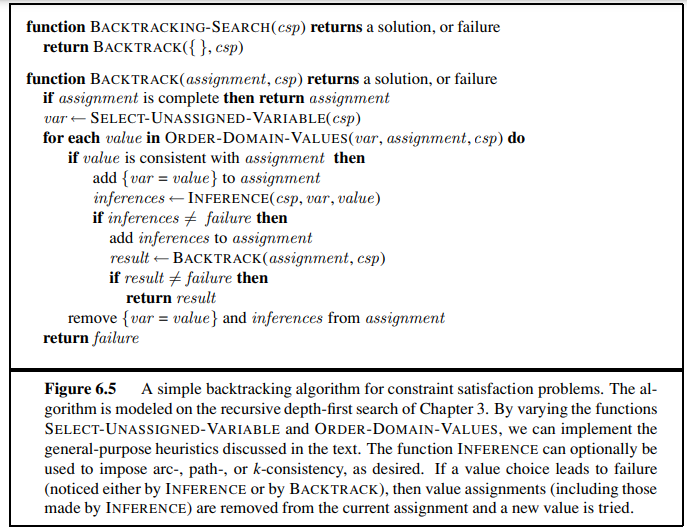
\includegraphics[scale=0.8]{images/CSP-backtracking.png}
\end{center}
The algorithm above implements backtracking search. It repeatedly chooses an unassigned variable, and then tries all values in the domain of that variable in turn, trying to find a solution. If an inconsistency is detected, then BACKTRACK returns failure, causing the previous call to try another value.\\\\
In the previous chapters we improved the poor performance of uninformed search algorithms by supplying them with domain-specific heuristic functions derived from our knowledge of the problem. It turns out that we can solve CSPs efficiently without such domain-specific knowledge. Instead, we can add some sophistication to the unspecified functions in the algorithm presented above using them to address the following questions:
\begin{enumerate}
    \item Which variable should be assigned next?

    \item In what order should its values be tried?

    \item When the search arrives at an assignment that violates a constraint, can the search avoid repeating this failure?

    \item Can we take advantage of problem structure?
\end{enumerate}

\subsection{Variable and value ordering}
The simplest strategy for SELECT-UNASSIGNED-VARIABLE is to choose the variable with the fewest “legal” values. This technique is usually  called the \textbf{most constrained variable} heuristic.
\begin{center}
    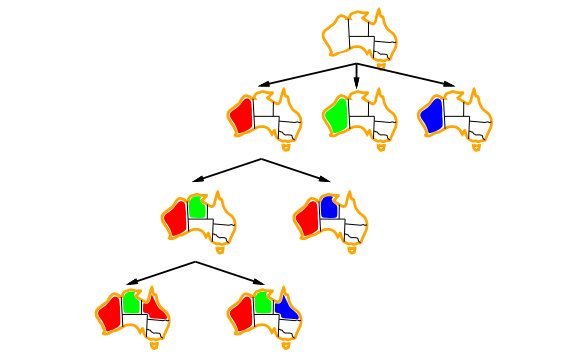
\includegraphics[scale=0.9]{images/CSP-MCV.png}
\end{center}
For example, in the figure above,  after the assignments for $WA = red$ and $NT = green$ (level 2) there is only one possible value for $SA$, so it makes sense to assign $SA = blue$ next rather than assigning $Q$.
\\\\
If some variable $X$ has no legal values left, the heuristic  will select $X$ and failure will be detected immediately, avoiding pointless searches through other variables (pruning the search tree). It usually performs better than a random or static ordering, sometimes by a factor of 1,000 or more, although the results vary widely depending on the problem.
\\\\
Once a variable has been selected, the algorithm must decide on the order in which to examine its values (ORDER-DOMAIN-VALUES). For this, the \textbf{least-constraining-value} heuristic can be effective in some cases.  It prefers the value that rules out the fewest choices for the neighboring variables in the constraint graph. For example, suppose that we have generated the partial assignment with $WA = red$ and $NT = green$ and that our next choice is for $Q$. Blue would
be a bad choice because it eliminates the last legal value left for $Q$’s neighbor, $SA$. The least-constraining-value heuristic therefore prefers red to blue.\\\\
Why should variable selection be fail-first, but value selection be fail-last?  It turns out that, for a wide variety of problems, a variable ordering that chooses a variable with the minimum number of remaining values helps minimize the number of nodes in the search tree by pruning larger parts of the tree earlier. For value ordering, the trick is that we only need one solution; therefore it makes sense to look for the most likely values first. If we wanted to enumerate all solutions rather than just find one, then value ordering would be irrelevant.

\subsection{Forward checking}
What inferences should be performed at each step in the search of the backtracking algorithm? The main idea behind \textbf{forward checking} is to keep track of remaining legal values for unassigned variables, terminating the search when any variable has no legal values. Whenever a variable $X$ is assigned, for each unassigned variable $Y$ that is connected to $X$ by a constraint, delete from $Y$ ’s domain any value that is inconsistent with the value chosen for $X$. By doing this, it eliminates branching on those values, making the search more efficient. Once forward checking detects that the partial assignment is inconsistent with the constraints of the problem, it backtracks immediately. Basically, it makes the backtracking algorithm more efficient preventing it from continuing the search when a partial assignment is inconsistent with the constraints of the problem.
\begin{center}
    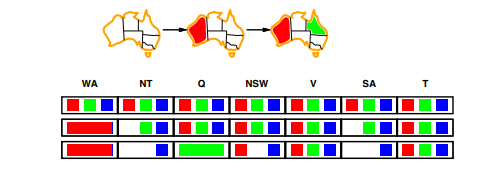
\includegraphics[]{images/CSP-forward-checking.png}
\end{center}
The figure above shows the progress of backtracking search on the Australia CSP with forward checking. There are two important points to notice about this example. First, notice that after $WA = red$ and $Q = green$ are assigned, the domains of $NT$ and $SA$ are reduced to a single value; we have eliminated branching on these variables altogether by propagating information from $WA$ and $Q$. A second point to notice is that after $V = blue$, the domain of $SA$ is empty. Hence, forward checking has detected that the partial assignment
$\{WA = red, Q = green, V = blue\}$ is inconsistent with the constraints of the problem, and the algorithm will therefore backtrack immediately.

\subsection{Constraint propagation}
Forward checking propagates information from assigned to unassigned variables, but doesn’t provide early detection for all failures. To solve this problem we can do a specific type of inference called \textbf{constraint propagation}:  using the constraints to reduce the number of legal values for a variable, which in turn can reduce the legal values for another variable, and so on. The key idea is \textbf{local consistency}. There are different types of local consistency, that we do not have time to discuss...

\subsection{Problem structure}
In this section, we examine ways in which the structure of the problem, as represented by the constraint graph, can be used to find solutions quickly.\\\\
Looking again at the constraint graph for Australia, one fact stands out: Tasmania is not connected to the mainland. Intuitively, it is obvious that coloring Tasmania and coloring the mainland are \textbf{independent sub-problems}. Independence can be ascertained simply by finding \textbf{connected components} of the constraint graph. Each component corresponds to a sub-problem.\\\\
Suppose each sub-problem has $c$ variables out of $n$ total, where $c$ is a constant. Then there are $n/c$ sub-problems, each of which takes at most $d^c$ work to solve, where $d$ is the size of the domain. Hence, the total work is $O(d^c n/c)$, which is linear in $n$. Without the decomposition, the total work is $O(d^n)$, which is exponential in $n$. Let’s make this more concrete: dividing a Boolean CSP with 80 variables into four sub-problems reduces the worst-case solution time from the lifetime of the universe down to less than a second.\\\\
Completely independent subproblems are delicious, then, but rare.  Fortunately, some
other graph structures are also easy to solve. For example, a constraint graph is a tree when any two variables are connected by only one path.\\\\
\textbf{Theorem:} if the constraint graph has no loops, the CSP can be solved in $O(nd^2)$ time.
\begin{center}
    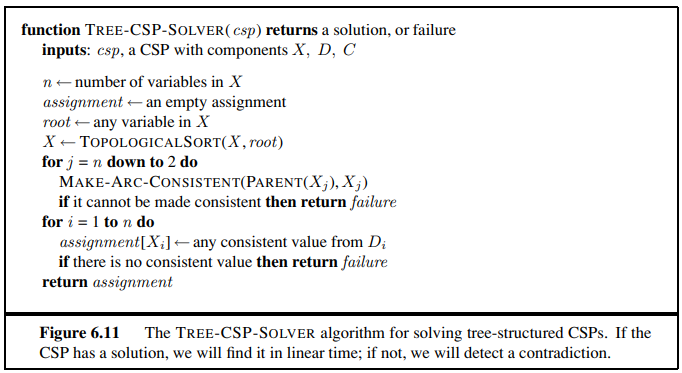
\includegraphics[]{images/CSP-Tree.png}
\end{center}

\section{Local search for CSPs}
Local search algorithms turn out to be effective in solving many CSPs. They
use a complete-state formulation: the initial state assigns a value to every variable, and the search changes the value of one variable at a time. The point of local search is to eliminate the violated constraints.\\\\
The next variable for an assignment is randomly selected within any conflicted variable. In choosing a new value for a variable, the most obvious heuristic is to select the value that results in the minimum number of conflicts with other variables, the \textbf{min-conflicts} heuristic. Min-conflicts is surprisingly effective for many CSPs. Amazingly, on the n-queens problem, if you don’t count the initial placement of queens, the run time of min-conflicts is roughly independent of problem size. It solves even the million-queens problem in an average of 50 steps (after the initial assignment).

